\documentclass[aspectratio=169]{beamer}
\usefonttheme{serif}
\usepackage{xeCJK}
\usepackage{fontspec}
\usepackage{graphicx}
\usepackage{listings}
\usepackage{xcolor}
\usepackage{indentfirst}
\usepackage{tikz}
\usepackage{amssymb}
\usepackage{amsthm}
\usepackage{amsmath}
\usepackage{tabularx}
\usepackage{hyperref}
\usepackage{ulem}
\usepackage{version}
\usepackage{thmtools}
\usepackage{qtree}
\usepackage{algpseudocode}
\usepackage{mathtools}
\usepackage{multicol}
\usepackage{xcolor}
\usepackage{ulem}

\AtBeginDocument{%
    \DeclareSymbolFont{pureletters}{T1}{lmr}{\mddefault}{it}%
}

\XeTeXlinebreaklocale "zh"
\XeTeXlinebreakskip = 0pt plus 1pt

\setCJKmainfont{NotoSansTC-Medium.otf}
\setmainfont{JetBrainsMono-SemiBold.ttf}

\usetikzlibrary{arrows,decorations.markings,decorations.pathreplacing}
\newenvironment{Hint}{\noindent\textbf{Hint.}}{}

\tikzstyle {graph node} = [circle, draw, minimum width=1cm]
\tikzset{edge/.style = {decoration={markings,mark=at position 1 with %
            {\arrow[scale=2,>=stealth]{>}}},postaction={decorate}}}

\lstset{
    basicstyle=\ttfamily\normalsize,
    numberstyle=\normalsize,
    numbers=left,
    stepnumber=1,
    numbersep=3pt,
    commentstyle=\color{black!50},
    keywordstyle=\color{white!0!blue},
    stringstyle=\color{black!50!green},
    showspaces=false,
    showstringspaces=false,
    showtabs=false,
    tabsize=4,
    captionpos=b,
    breaklines=true,
    breakatwhitespace=false,
    escapeinside={\%*}{*)},
    morekeywords={*}
}

\AtBeginSection[]{
  \begin{frame}
  \vfill
  \centering
  \begin{beamercolorbox}[sep=8pt,center,shadow=true,rounded=true]{title}
    \usebeamerfont{title}\insertsectionhead\par%
  \end{beamercolorbox}
  \vfill
  \end{frame}
}

\title{貪心與基礎證明技巧}
\author{sam571128}
\date{2022-07-04}

\usetheme{Madrid}
\usecolortheme{default}
\setbeamertemplate{itemize items}[square]
\setbeamertemplate{enumerate items}[default]
\setbeamertemplate{blocks}[default]

\begin{document}

\frame{\titlepage}

\begin{frame}
\frametitle{所以這堂課要上什麼?}
    \begin{itemize}
    \item<1-> 貪心? 那是什麼?
    \item<2-> 不要擔心,讓我們先來看看一個情境
    \end{itemize}
\end{frame}

\begin{frame}
\frametitle{所以這堂課要上什麼?}
    \begin{block}{找零錢}
    今天,你走進一間便利商店,你總共買了總價錢為新台幣 $456$ 元 的商品,不過你手邊剛好沒有足夠的零錢,只有一張 $1000$ 元紙鈔。請問店員最少要拿多少鈔票與硬幣才能完成找錢?
    \end{block}
    \begin{itemize}
    \item<1-> 我們先計算出要找的錢為 $1000 - 456 = 544$ 元
    \item<2-> 接著,應該會直接拿取 $1$ 張 $500$、$4$ 個 $10$ 元、以及 $4$ 個 $1$ 元
    \item<3-> 所以只要拿 $8$ 個就好,而這也是最小的答案
    \item<4-> \sout{恭喜你,學會貪心了! 我們下課吧}
    \end{itemize}
\end{frame}

\begin{frame}
\frametitle{貪心到底是什麼?}
    \begin{itemize}
    \item<1-> 在剛剛那個題目中,我們做了什麼?
    \item<2-> 我們很直覺的認為,只要一路選擇最大面額,就可以選到最少的零錢了!
    \item<3-> 事實上,上面在做的事情其實就是貪心演算法!
    \item<4-> 我們照著這樣子的策略,每次都拿可以拿的最大面額,最終得到最小的答案
    \item<5-> 這個就被我們稱為「貪心」
    \end{itemize}
\end{frame}

\begin{frame}
\frametitle{貪心到底是什麼?}
    \begin{itemize}
    \item<1-> 在日常生活中,我們時常在不經意的時候就會使用到貪心
    \item<2-> 例如剛剛的找零問題,一般人都會有著要用最大面額開始換的想法
    \item<3-> 不過,照著直覺走一定會是最好的嗎?
    \end{itemize}
\end{frame}

\begin{frame}
\frametitle{貪心真的是對的嗎?}
    \begin{block}{換零錢}
    今天,你在一個某國旅遊,該國的硬幣面額為 $v_1, v_2, \ldots, v_n$ ,而你經過了一個商店,你總共買了總價錢為 $x$ 元 的商品,請問你最少要拿幾個硬幣才能湊出 $x$ 元。
    \end{block}
    
    \begin{itemize}
    \item<1-> 這個問題與剛剛有什麼不同呢?
    \item<1-> 照著我們剛剛的策略會得到最少的答案嗎?
    \item<3-> 大家可以試著思考看看
    \end{itemize}
\end{frame}

\begin{frame}
\frametitle{貪心真的是對的嗎?}
    \begin{block}{換零錢}
    今天,你在一個某國旅遊,該國的硬幣面額為 $v_1, v_2, \ldots, v_n$ ,而你經過了一個商店,你總共買了總價錢為 $x$ 元 的商品,請問你最少要拿幾個硬幣才能湊出 $x$ 元。
    \end{block}
    
    \begin{itemize}
    \item<1-> 我們隨意將變數換成實際的數字來想想看
    \item<2-> 假設面額是 $1,5,8$,而 $x=15$?
    \item<3-> 此時,我們會發現,如果照著剛剛的策略走,會拿到 $\{8,5,1,1\}$,但最少的答案只需要選取 $\{5,5,5\}$
    \item<4-> 這樣的策略不是正確的?
    \end{itemize}
\end{frame}

\begin{frame}
\frametitle{貪心真的是對的嗎?}
    \begin{itemize}
    \item<1-> 從上面那個例子,我們可以知道,靠著直覺走,貪心的做法並不會每次皆是正確的
    \item<2-> 那我們又為什麼需要使用這樣子的方式呢?
    \item<3-> 貪心演算法雖然不見得是正確的,但通常比起一般的作法來得更有效率
    \item<4-> 在本堂課的最後,會教大家一些證明演算法正確性的方式
    \end{itemize}
\end{frame}

\begin{frame}
\frametitle{貪心的步驟}
    \begin{itemize}
    \item<1-> 我們在解題時,也會經常遇到與貪心相關的問題,我將其分為三個步驟
    \item<1-> 「觀察」、「嘗試」、「驗證」
    \end{itemize}
\end{frame}

\begin{frame}
\frametitle{貪心的步驟}
    \begin{alertblock}{第一步、觀察}
        觀察題目的情境,看看有什麼是我們策略是我們可以照著做的,並試著猜測看看
    \end{alertblock}
    
    \begin{itemize}
    \item<1-> 此步驟通常是最關鍵的一步,在簡單的題目中,貪心策略通常滿直覺的
    \end{itemize}
\end{frame}

\begin{frame}
\frametitle{貪心的步驟}
    \begin{alertblock}{第二步、嘗試}
        觀察完題目後,得到了我們猜測的策略。我們可以試著想想各種不同的情況或測資,試著去尋找是否有能使該策略產生錯誤答案的可能性
    \end{alertblock}
\end{frame}

\begin{frame}
\frametitle{貪心的步驟}
    \begin{alertblock}{第三步、驗證}
        實際的使用數學證明,嚴謹的去證明該算法的正確性
    \end{alertblock}
    
    \begin{itemize}
    \item<1-> 此步驟十分重要,但是在比賽中,許多人會省略這個步驟,直接 Proof By AC
    \item<1-> 不過建議大家,即使在比賽中猜測出了正確做法,還是可以自己練習證明看看
    \item<2-> 本堂課前面會先略過證明的部分,在介紹證明時一併證明
    \end{itemize}
\end{frame}

\section{貪心法經典題}

\begin{frame}
\frametitle{貪心法經典題(一)}
    \begin{block}{活動安排問題 (CSES - Movie Festival)}
        Colten 想要看電影,他知道總共有$n$場電影可以看。而每場電影會從時間點 $l_i$ 開始播映到時間點 $r_i$。在同一個時間點,Colten 沒有辦法同時看兩部電影(不過如果有一部電影在時間點 $x$ 結束播映,Colten 還是可以去看時間點 $x$ 開始播映的電影),請問 Colten 最多可以看幾部電影?
    \end{block}
    
    \begin{itemize}
    \item<1-> 這題我們讓大家先想想看,看看有沒有人有什麼想法
    \end{itemize}
\end{frame}

\begin{frame}
\frametitle{貪心法經典題(一)}
    \begin{block}{活動安排問題 (CSES - Movie Festival)}
        Colten 想要看電影,他知道總共有$n$場電影可以看。而每場電影會從時間點 $l_i$ 開始播映到時間點 $r_i$。在同一個時間點,Colten 沒有辦法同時看兩部電影(不過如果有一部電影在時間點 $x$ 結束播映,Colten 還是可以去看時間點 $x$ 開始播映的電影),請問 Colten 最多可以看幾部電影?
    \end{block}
    
    \begin{itemize}
    \item<1-> 一個滿直覺的想法,既然想要看最多的電影,那我們從開始時間最早的電影開始看呢?
    \end{itemize}
\end{frame}

\begin{frame}
\frametitle{貪心法經典題(一)}
    \begin{itemize}
    \item<1-> 一個滿直覺的想法,既然想要看最多的電影,那我們從開始時間最早的電影開始看呢?
    \end{itemize}
    
    \begin{center}
        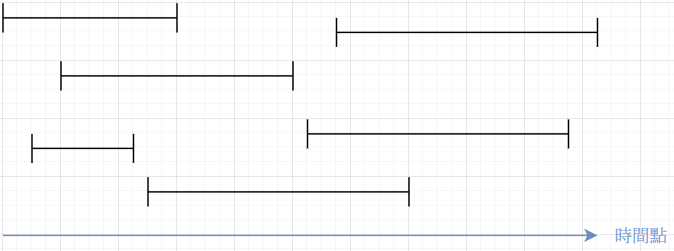
\includegraphics[scale=0.75]{images/movie_festival_1.png}
    \end{center}
\end{frame}

\begin{frame}
\frametitle{貪心法經典題(一)}
    \begin{itemize}
    \item<1-> 根據這些電影的時段,我們根據剛剛的想法,會選出畫成紅色的這兩部電影
    \end{itemize}
    
    \begin{center}
        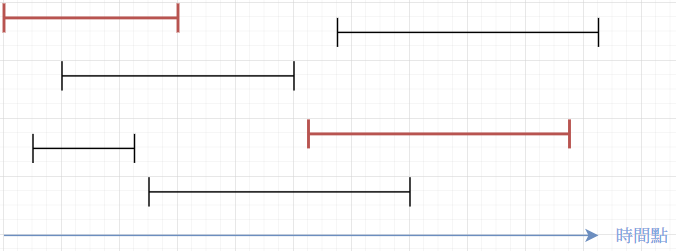
\includegraphics[scale=0.75]{images/movie_festival_2.png}
    \end{center}
\end{frame}

\begin{frame}
\frametitle{貪心法經典題(一)}
    \begin{itemize}
    \item<1-> 接著,我們會發現,這其實是最多的答案,我們找不到更好的答案了!
    \end{itemize}
    
    \begin{center}
        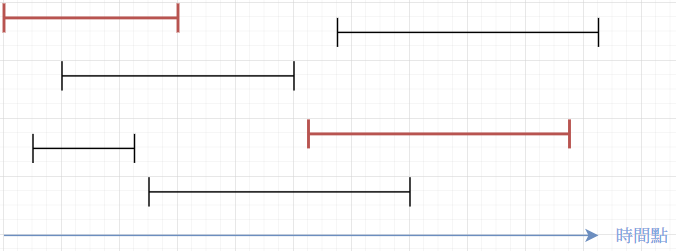
\includegraphics[scale=0.75]{images/movie_festival_2.png}
    \end{center}
\end{frame}

\begin{frame}
\frametitle{貪心法經典題(一)}
    \begin{itemize}
    \item<1-> 因此對於這個題目,我們可以將第一步寫出來
    \end{itemize}
    
    \begin{alertblock}{第一步、觀察}
        根據題目所述,從開始放映時間最早的電影開始看,好像可以得到最佳的答案
    \end{alertblock}
\end{frame}


\begin{frame}
\frametitle{貪心法經典題(一)}
    \begin{itemize}
    \item<1-> 第一個步驟出來之後,我們要經過多次嘗試,才能說服我們他會是對的!
    \item<2-> 因此,我們可以再找幾組電影的播映時間來測試這個想法是否正確。
    \end{itemize}
\end{frame}

\begin{frame}
\frametitle{貪心法經典題(一)}
    \begin{center}
        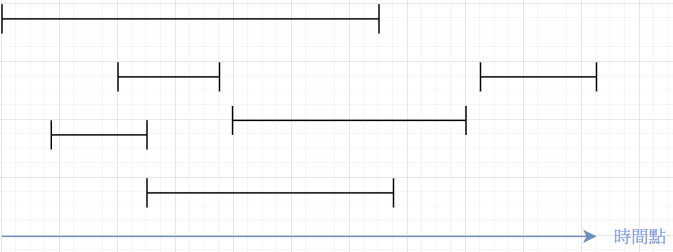
\includegraphics[scale=0.75]{images/movie_festival_3.png}
    \end{center}
\end{frame}

\begin{frame}
\frametitle{貪心法經典題(一)}
    \begin{center}
        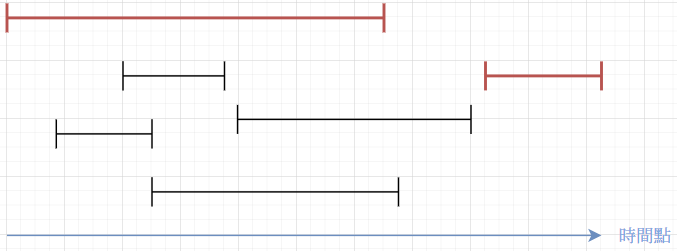
\includegraphics[scale=0.75]{images/movie_festival_4.png}
    \end{center}
    
    \begin{itemize}
    \item<1-> 根據剛剛的策略,我們知道 Colten 最多能看 $2$ 部電影 (嗎? 
    \end{itemize}
\end{frame}

\begin{frame}
\frametitle{貪心法經典題(一)}
    \begin{center}
        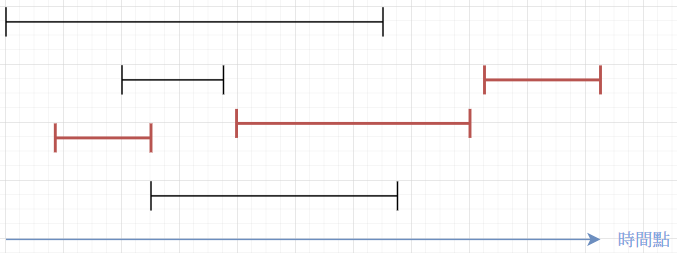
\includegraphics[scale=0.75]{images/movie_festival_5.png}
    \end{center}
    
    \begin{itemize}
    \item<1-> 換一種方式畫的話,最多能看 $3$ 部欸!
    \end{itemize}
\end{frame}

\begin{frame}
\frametitle{貪心法經典題(一)}
    \begin{itemize}
    \item<1-> 因此我們在第二步時,成功的發現了這個做法並不會每次都是正確的
    \item<2-> 那有沒有別的想法呢?
    \end{itemize}
\end{frame}

\begin{frame}
\frametitle{貪心法經典題(一)}
    \begin{itemize}
    \item<1-> 換一個想法,既然看最早開始的行不通,那我們從最早結束的開始看,是不是能夠留給我們更多看後面電影的時間呢?
    \end{itemize}
    \begin{alertblock}{第一步、觀察}
        根據題目所述,從結束放映時間最早的電影開始看,好像可以得到最佳的答案
    \end{alertblock}
\end{frame}

\begin{frame}
\frametitle{貪心法經典題(一)}
    \begin{itemize}
    \item<1-> 使用剛剛的例子來看一次
    \end{itemize}
    \begin{center}
        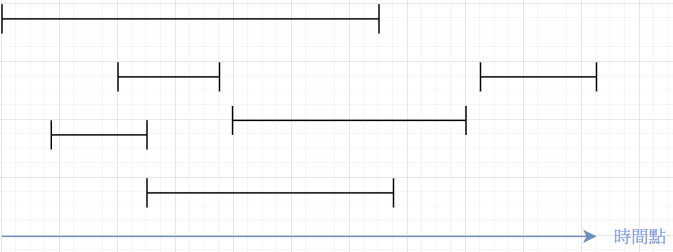
\includegraphics[scale=0.75]{images/movie_festival_3.png}
    \end{center}
\end{frame}

\begin{frame}
\frametitle{貪心法經典題(一)}
    \begin{itemize}
    \item<1-> 欸? 答案好像是對的欸!
    \end{itemize}
    \begin{center}
        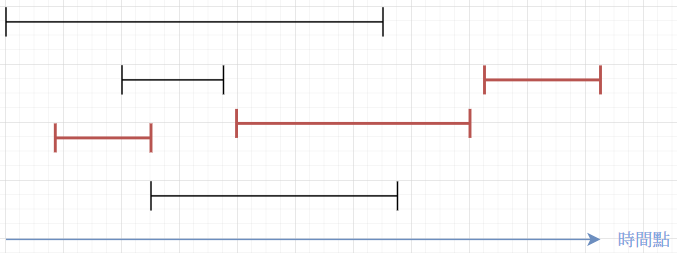
\includegraphics[scale=0.75]{images/movie_festival_5.png}
    \end{center}
\end{frame}

\begin{frame}
\frametitle{貪心法經典題(一)}
    \begin{itemize}
    \item<1-> 事實上,這題的正確做法確實就是這樣沒有錯! \pause
    \item<2-> 不論你經過多少次的嘗試,這個作法皆會產生正確的答案! \pause
    \item<3-> 因此,這個做法通過了我們「嘗試」的考驗 \pause
    \end{itemize} 
    
    \begin{alertblock}{第二步、嘗試}
        根據多次的嘗試,我們只要從結束放映時間最早的電影開始看,皆能正確的產生答案
    \end{alertblock}
\end{frame}

\begin{frame}
\frametitle{貪心法經典題(一)}
    \begin{itemize}
    \item<1-> 使用這個例子是想告訴大家,在寫貪心的題目時,如果你有辦法得到任意一組能夠使貪心法產生錯誤答案的方法,則該方法就會是錯誤的!
    \item<2-> 不過另外一個要提醒的一點是,儘管經過了多次嘗試皆無法證明貪心法是錯誤的,我們還是必須要牢記,我們還沒有進行「驗證」,或者說實際的去證明這個方法的正確性
    \item<2-> 而這些題目的證明,我會留在本堂課的最後一併進行證明
    \end{itemize}
\end{frame}

\begin{frame}
\frametitle{貪心法經典題(二)}
    \begin{block}{誰先晚餐 (TIOJ 1072)}
        Colten 與他的朋友們一共 $n$ 個人前往某間餐廳吃午餐,不過這間餐廳只有一個人可以準備大家所要吃的餐點,也就是說在同一個時間,他只能準備一個人點的餐點。第 $i$ 個人所點的餐點需要 $a_i$ 的時間準備,並且他需要 $b_i$ 的時間才能吃完他們所點的食物。請問總共最少需要多少時間才能讓所有人都吃完他們所點的餐點?
        
        測資範圍: $n \le 10^5$
    \end{block}
    \begin{itemize}
        \item<2-> 這個題目看上去好困難喔,我們可以先把問題想的簡單一點,其實我們只需要決定好廚師要先煮誰的餐點即可!
        \item<3-> 大家可以試著想想看,這個問題我們應該如何處理
    \end{itemize}
\end{frame}

\begin{frame}
\frametitle{貪心法經典題(二)}
    \begin{itemize}
        \item<1-> 接著,又來到了我們猜測做法的時間了! \pause
        \item<2-> 如果,我們照著餐點準備的時間由慢到快去排順序呢? \pause
    \end{itemize}
    
    \begin{alertblock}{第一步、觀察}
        照著餐點準備的時間決定要先煮誰的餐點,好像可以得到正確的答案 
    \end{alertblock}
\end{frame}

\begin{frame}
\frametitle{貪心法經典題(二)}
    \begin{itemize}
        \item<1-> 欸? 範測過了!
        \item<2-> 自己寫出一些可能性來觀察看看!
    \end{itemize}
\end{frame}

\begin{frame}
\frametitle{貪心法經典題(二)}
    \begin{itemize}
        \item<1-> 經過嘗試後,我們發現這個想法是錯的! \pause
        \item<2-> 如果有一個人的餐點準備時間很長,但他吃的時間很慢,是不是就會導致總時間花了很久? \pause
    \end{itemize}
    
    \begin{center}
        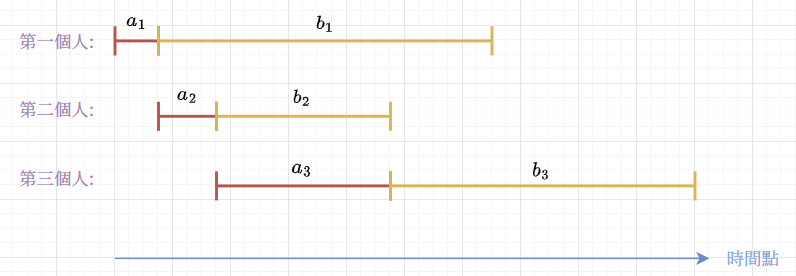
\includegraphics[scale=0.7]{images/dinner_1.png}
    \end{center}
\end{frame}

\begin{frame}
\frametitle{貪心法經典題(二)}
    \begin{itemize}
        \item<1-> 我們會發現,吃飯的時間影響也很大! 
        \item<2-> 那麼,我們就讓吃最慢的人先吃不就好了!
    \end{itemize}
\end{frame}

\begin{frame}
\frametitle{貪心法經典題(二)}
    與剛剛相同的 $a_i,b_i$,使用了不同策略的結果
    
    \begin{center}
        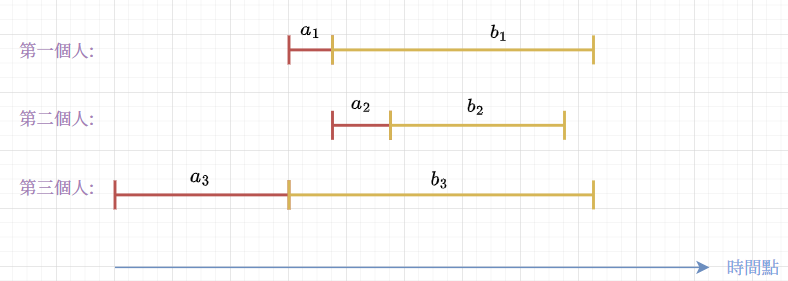
\includegraphics[scale=0.7]{images/dinner_2.png}
    \end{center}
\end{frame}

\begin{frame}
\frametitle{貪心法經典題(二)}
    因此,我們得到了一個可以解決這題的方法!
    \begin{alertblock}{第二步、嘗試}
        根據多次的嘗試,照著吃飯速度決定要先煮誰的餐點,都可以產生正確的答案
    \end{alertblock}
\end{frame}

\begin{frame}
\frametitle{貪心法經典題(三)}
    \begin{block}{CSES - Tasks and Deadline}
        Colten 有 $n$ 個任務要完成,而對於第 $i$ 個任務,他的期限為第 $d_i$ 天,Colten 需要 $a_i$ 的時間才能完成。當 Colten 在第 $f$ 天完成第 $i$ 個任務時,他會得到 $d_i-f_i$ 的報酬 (在期限後完成的話,報酬可能會是負的),請問 Colten 最多能獲得多少報酬?
    \end{block}
    \begin{itemize}
        \item<1-> 這題我們給大家一點時間想想看,看看有沒有人有什麼想法
    \end{itemize}
\end{frame}

\begin{frame}
\frametitle{貪心法經典題(三)}
    \begin{block}{CSES - Tasks and Deadline}
        Colten 有 $n$ 個任務要完成,而對於第 $i$ 個任務,他的期限為第 $d_i$ 天,Colten 需要 $a_i$ 的時間才能完成。當 Colten 在第 $f$ 天完成第 $i$ 個任務時,他會得到 $d_i-f_i$ 的報酬 (在期限後完成的話,報酬可能會是負的),請問 Colten 最多能獲得多少報酬?
    \end{block}
    \begin{itemize}
        \item<1-> 這個應該也是個滿生活化的例子吧!
        \item<2-> 在生活中,我們會選擇什麼樣的方法來完成我們手上的任務呢?
        \item<3-> 依照期限短的先做吧!
    \end{itemize}
\end{frame}

\begin{frame}
\frametitle{貪心法經典題(三)}
    \begin{itemize}
        \item<1-> 欸? 範測錯了!
        \item<2-> 照著期限短的先處理居然不是最好的嗎?
    \end{itemize}
    
    \begin{center}
        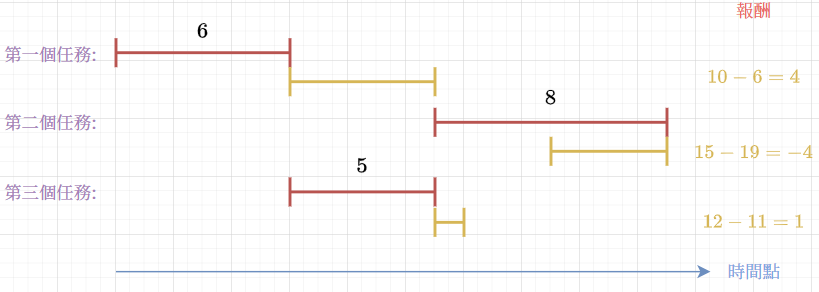
\includegraphics[scale=0.7]{images/tasks_and_deadline_1.png}
    \end{center}
\end{frame}

\begin{frame}
\frametitle{貪心法經典題(三)}
    \begin{itemize}
        \item<1-> 以這題為例子,我們可以發現,直覺的作法不見得每次都會是正確的!
        \item<2-> 那我們再來猜猜看,這題正確的做法究竟是如何呢?
        \item<3-> 依照完成時間來做做看呢?
    \end{itemize}
\end{frame}

\begin{frame}
\frametitle{貪心法經典題(三)}
    依照完成時間排序範測得到的結果
    
    \begin{center}
        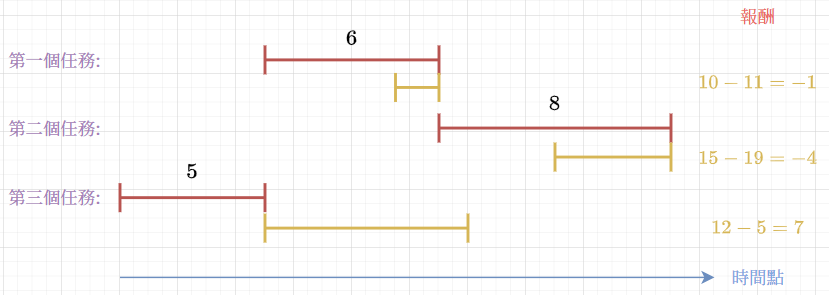
\includegraphics[scale=0.68]{images/tasks_and_deadline_2.png}
    \end{center}
\end{frame}

\begin{frame}
\frametitle{貪心法經典題(三)}
    \begin{itemize}
        \item<1-> 好像是對的欸! 我們實際將解丟到 judge 上看看吧!
        \item<2-> AC! 但是.... 為什麼呢?
        \item<3-> 我們發現了,直覺不會總是帶給我們正確的答案,這種 Proof By AC 的方式並不是嚴謹的!
        \item<4-> 因此,讓我們實際學習一些證明的方法後,再回來看看這些方法的正確性吧
    \end{itemize}
\end{frame}
    
\begin{frame}
\frametitle{練習題}
    \begin{block}{數字合併問題 (類似題: CSES - Stick Division)}
        Alice 和 Bob 在玩遊戲,Alice 會在黑板上寫下 $n$ 個數字,而 Bob 每次可以選擇兩個數字 $a, b$,將他們從黑板上擦掉,得到 $a+b$ 的分數,並在黑板上寫下 $a+b$,現在你知道 Alice 寫下的 $n$ 個數字是哪 $n$ 個,請問 Bob 最多可以得到多少分數?
    \end{block}
    \begin{block}{NHDK Ten Point Round \#20 pG - 隊伍編排}
        有 $n$ 個人要排隊,第 $i$ 個人有一個容忍度 $a_i$ 與一個包容度 $b_i$,對於兩個人 $x,y$,如果 $x$ 排在 $y$ 的前面,$x$ 就會增加 $b_x (b_x-2) - a_y (a_y+5)$ 的煩躁度,這些人可以任意排列,問所有人的煩躁度總和最小可以是多少?
    \end{block}
\end{frame}

\begin{frame}
\frametitle{練習題}
    \begin{block}{最大子陣列和(CSES - Maximum Subarray Sum)}
        給你一個 $n$ 項的陣列 $(n \le 10^5)$,請問對於所有子陣列(陣列中一段連續的數字),最大的總和為何?
    \end{block}
    \begin{block}{NEOJ 90 - 調校高棕櫚! (資訊之芽貪心上機作業)}
        你有 $n$ 個保鮮盒與 $m$ 個高棕櫚,第 $i$ 個高棕櫚有一個成熟度 $F_i$,你可以將高棕櫚分裝到不同的保鮮盒當中,而第 $i$ 保鮮盒所裝的高棕櫚的成熟度總和不能超過 $M_i$,請問你最多能夠用這 $n$ 個保鮮盒裝多少高棕櫚回家?
        
        測資範圍: 
        \begin{itemize}
            \item $1 \le n,m \le 10^5$
            \item $1 \le F_i, M_i \le 10^6$
            \item 高棕櫚的成熟度互相存在倍數關係
        \end{itemize}
    \end{block}
\end{frame}

\section{基礎證明技巧}
    
\begin{frame}
\frametitle{證明方法}
    \begin{itemize}
        \item<1-> 在此的學員,大多數應該都對於離散數學的證明都不太熟悉
        \item<1-> 以台灣的數學教育來說,大部分人應該只學過幾何的證明(全等、相似三角形) 
        \item<1-> 不過對於資訊方面來說,證明的方法可能與以前所遇到的都不同
        \item<1-> 接下來的內容可能會比較無聊,但是對於我們看懂貪心的證明來說十分重要!
        \item<2-> 這裡會介紹幾種不同的證明方法
    \end{itemize}
\end{frame}

\begin{frame}
\frametitle{證明方法(一)- 反證法 (Proof by Contradiction)}
    \begin{itemize}
        \item<1-> 首先,在證明演算法時,尤其是貪心演算法,最常用到的就是反證法
        \item<2-> 如果我們想要證明某個命題是錯誤的,那我們先假設他是對的
        \item<2-> 當這個假設發生矛盾時,我們就可以說該命題是錯的了!
        \item<3-> 有點難懂? 沒關係,我們來看看實際例子
    \end{itemize}
\end{frame}

\begin{frame}
\frametitle{證明方法(一)- 反證法 (Proof by Contradiction)}
    \begin{block}{證明 $\sqrt{2}$ 是無理數}
        請證明 $\sqrt{2}$ 是一個無理數,意即我們無法用兩個互質的整數 $p,q$,將其表示為 $\frac{p}{q}$。
    \end{block}
    
    \begin{itemize}
        \item<1-> 這個題目在高中時大家應該都學過了! 利用到的就是反證法!
    \end{itemize}
\end{frame}

\begin{frame}
\frametitle{證明方法(一)- 反證法 (Proof by Contradiction)}
    \begin{block}{證明 $\sqrt{2}$ 是無理數}
        請證明 $\sqrt{2}$ 是一個無理數,意即我們無法用兩個互質的整數 $p,q$,將其表示為 $\frac{p}{q}$。
    \end{block}
    
    假設 $\sqrt{2}$ 是一個有理數,可以寫出 
    $$\sqrt{2}=\frac{p}{q}$$
    將兩邊進行平方與移項後
    $$2q^2 = p^2$$
    則我們可以知道 $p$ 一定是 $2$ 的倍數。令 $p=2k$,式子變為
    $$2q^2 = (2k)^2 = 4k^2 \rightarrow q^2=2k^2$$
    $q$ 一定也是 $2$ 的倍數,因此 $p,q$ 不可能互質,所以 $\sqrt{2}$ 不可能是無理數 \\
    以反證法得證。
\end{frame}

\begin{frame}
\frametitle{證明方法(一)- 反證法 (Proof by Contradiction)}
    \begin{block}{證明一個群體當中,一定有兩個人認識的人數相同}
        在一個有 $n (n \ge 1)$ 個人的群體當中,任意兩人可能互相認識或互相不認識,請證明這個群體必定存在兩個人認識的人數一樣多。
    \end{block}
    \begin{itemize}
        \item 這題給大家想想看,我們要怎麼證明這題呢?
    \end{itemize}
\end{frame}

\begin{frame}
\frametitle{證明方法(一)- 反證法 (Proof by Contradiction)}
    \begin{block}{證明一個群體當中,一定有兩個人認識的人數相同}
        在一個有 $n (n \ge 1)$ 個人的群體當中,任意兩人可能互相認識或互相不認識,請證明這個群體必定存在兩個人認識的人數一樣多。
    \end{block}
    假設任兩個人認識的人數都不同。則每個人認識的人數分別會是 $0,1,\ldots,n-1$,不過我們知道,如果其中有一個人認識的人數為 $0$,意即沒有朋友,則不可能會有人認識 $n-1$ 個人,意即認識除了自己以外的所有人,產生矛盾。根據鴿籠原理,該群體必定存在兩個人認識的人數一樣多。以反證法得證。
\end{frame}

\begin{frame}
\frametitle{證明方法(一)- 反證法 (Proof by Contradiction)}
    反證法的步驟大概如下
    \begin{enumerate}
        \item 對於一個想要證明正確性的命題,先假設他是錯誤的
        \item 根據這個假設去進行推論
        \item 如果產生矛盾,表示命題為真
    \end{enumerate}
\end{frame}

\begin{frame}
\frametitle{證明方法(二)- 數學歸納法 (Mathematical Induction)}
    \begin{itemize}
        \item 這個證明方法比起前一個反證法,各位應該更加熟悉
        \item 在高中的數學課中,相信大家都已經學過這個證明方法了
        \item 不過,在證明演算法時,數學歸納法是一個十分常用的證明方式
    \end{itemize}
\end{frame}

\begin{frame}
\frametitle{證明方法(二)- 數學歸納法 (Mathematical Induction)}
    對於一個命題 $P(n)$,如果要證明對於所有 $n$,$P(n)$ 皆為真,步驟如下
    \begin{enumerate}
        \item 先確認邊界條件成立
        \item 假設對於所有 $i \le k$,$P(i)$ 皆為真
        \item 我們可以利用 $P(i)$ 推論出 $P(i+1)$ 也會是對的
        \item 則對於所有數字 $n$,$P(n)$ 皆會成立
    \end{enumerate} \pause
    讓我們實際來看看一些例題
\end{frame}

\begin{frame}
\frametitle{證明方法(二)- 數學歸納法 (Mathematical Induction)}
    \begin{block}{證明 $\sum i^2$ 的總和}
        請證明 $\sum_{i=1}^n i^2$ 的總和是 $\frac{n(n+1)(2n+1)}{6}$
    \end{block}
    
    \begin{enumerate}
        \item<1-> 對於 $n=1$ 時,$1^2 = \frac{1 \times 2 \times 3}{6}$,成立
        \item<2-> 假設對於 $n = k$ 時成立,則 $\sum_{i=1}^{k} i^2 = \frac{k(k+1)(2k+1)}{6}$
        \item<3-> 則我們可以對上式左右兩邊加上 $k^2$,對於 $n=k+1$,我們可以得到 $$\sum_{i=1}^{k-1} i^2 + (k+1)^2 = \frac{k(k+1)(2k+1)}{6} + (k+1)^2 = \frac{(k+1)(k+2)(2k+3)}{6}$$
        \item<4-> 由數學歸納法得證。
    \end{enumerate}
\end{frame}

\begin{frame}
\frametitle{證明方法(二)- 數學歸納法 (Mathematical Induction)}
    \begin{block}{證明遞迴的時間複雜度! (遞迴算費氏數列,時間複雜度 $\in  O(2^n)$)}
        請證明對於下列函數滿足 $f(x) \le 2^x$
        $$f(x) = \begin{cases} 
                 1  & x \le 2 \\
                 f(x-1)+f(x-2) & x > 2 \\
               \end{cases}$$
    \end{block}
\end{frame}

\begin{frame}
\frametitle{證明方法(二)- 數學歸納法 (Mathematical Induction)}
    \begin{block}{證明遞迴的時間複雜度! (遞迴算費氏數列,時間複雜度 $\in O(2^n)$)}
        請證明對於下列函數滿足 $f(x) \le 2^x$
        $$f(x) = \begin{cases} 
                 1  & x \le 1 \\
                 f(x-1)+f(x-2) & x > 1 \\
               \end{cases}$$
    \end{block}
    
    \begin{enumerate}
        \item<1-> 對於 $n=0$ 時,$f(0) = 1 \le 2^0$,成立
        \item<1-> 對於 $n=1$ 時,$f(1) = 1 \le 2^1$,成立
        \item<2-> 假設對於 $n = k$ 與 $n=k+1$ 時成立,則 $f(k) \le 2^k$ 且 $f(k+1) \le 2^{k+1}$
        \item<3-> 則對於 $n=k+2$,我們可以得到 $f(k)+f(k+1) \le 2^k+2^{k+1} = 2^k(1+2) < 2^{k+2}$
        \item<4-> 由數學歸納法得證。
    \end{enumerate}
\end{frame}

\begin{frame}
\frametitle{證明方法(二)- 數學歸納法 (Mathematical Induction)}
    \begin{itemize}
        \item<1-> 剛剛看的例子是我們證明遞迴的時間複雜度的其中一種
        \item<1-> 在之後的課程介紹到分治時,我們也可以使用數學歸納法的方式去證明他的時間複雜度
        \item<2-> 數學歸納法的好處就是我們不用知道一個式子是怎麼來的,只要猜測答案之後嘗試數歸就好!這個是不是跟貪心的作法很像呢?
    \end{itemize}
\end{frame}

\begin{frame}
\frametitle{證明方法(三)- 構造性證明 (Constructive Proof)}
    \begin{itemize}
        \item<1-> 與前面兩種方法比較不同的是,這個方法我們會實際創造出一個例子
        \item<2-> 通常會與存在性的證明有關,構造出一組解或一種方案就可以證明了!
    \end{itemize}
\end{frame}

\begin{frame}
\frametitle{證明方法(三)- 構造性證明 (Constructive Proof)}
    \begin{block}{證明奇數可以被寫成完全平方數的差}
        請證明任何一個奇數 $x$ 皆可以被寫成兩個完全平方數的差
    \end{block}
\end{frame}

\begin{frame}
\frametitle{證明方法(三)- 構造性證明 (Constructive Proof)}
    \begin{block}{證明奇數可以被寫成完全平方數的差}
        請證明任何一個奇數 $x$ 皆可以被寫成兩個完全平方數的差
    \end{block}
        
    我們可以假設 $a=k+1, b=k$,則 $$a^2-b^2 = (k+1)^2-k^2 = 2k+1$$
    令 $x=2k+1$。對於任意奇數 $x$,皆可以找到 $$a=\frac{x-1}{2}+1, b=\frac{x-1}{2}$$ 
    使得 $a^2-b^2=x$,得證。
\end{frame}

\begin{frame}
\frametitle{證明方法(三)- 構造性證明 (Constructive Proof)}
    \begin{block}{證明質數有無限多個}
        請證明質數的數量有無限多個。
    \end{block}
\end{frame}

\begin{frame}
\frametitle{證明方法(三)- 構造性證明 (Constructive Proof)}
    \begin{block}{證明質數有無限多個}
        請證明質數的數量有無限多個。
    \end{block}
    假設我們已經知道質數只有 $k$ 個 $p_1, p_2, \ldots, p_k$,則我們可以構造一個數字 $$x = p_1p_2\ldots p_k + 1$$使其與這 $k$ 個質數皆互質,以此方式進行構造,則 $x$ 本身必為質數或者有並非在這 $k$ 個質數中的質因數,由此可知質數的數量不只 $k$ 個,得證。
\end{frame}


\begin{frame}
\frametitle{證明方法}
    \begin{itemize}
        \item 在介紹完了那麼多證明方法之後,我們接著就要實際來將他們運用在貪心的演算法當中了
        \item 本節在介紹這些證明方法時,想必有許多學員已經感到十分疲累了
        \item 這些證明方法對於未來要就讀資工系的大家是滿重要的技能
        \item 希望能夠幫助大家對於資訊方面的證明方法有更加的了解
    \end{itemize}
\end{frame}

\begin{frame}
\frametitle{練習題}
    \begin{block}{證明 $\sqrt[3]{5}$ 是無理數}
        請證明 $\sqrt[3]{5}$ 是無理數。
    \end{block}
    
    \begin{block}{證明 $\sum_{i=1}^n i \cdot 2^{i-1} = 2^n \cdot (n-1) + 1$}
        請證明 $\sum_{i=1}^n i \cdot 2^{i-1} = 2^n \cdot (n-1) + 1$。
    \end{block}
    
    \begin{block}{鴿籠原理?}
        給你一個 $9 \times 9$ 的網格圖,每個格子裡面有一隻鴿子,下一秒,這些鴿子會往原本格子的四個方向移動一格,但他們不能離開 $9 \times 9$ 的範圍。請證明下一秒,一定有兩個鴿子共用同一個格子。
    \end{block}
\end{frame}

\section{貪心法的證明}

\begin{frame}
\frametitle{回到貪心法}
    \begin{itemize}
        \item 看完那麼多數學證明,那我們來實際使用那些方式來證明看看貪心吧!
        \item 第一個例題就是我們最一開始講過的「換零錢」問題
    \end{itemize} \pause
    
    \begin{block}{換零錢}
    今天,你在一個某國旅遊,該國的硬幣面額為 $v_1, v_2, \ldots, v_n$ ,而你經過了一個商店,你總共買了總價錢為 $x$ 元 的商品,請問你最少要拿幾個硬幣才能湊出 $x$ 元。 \\
    測資限制: $v_1 = 1, v_i | v_{i+1}$ (也就是說 $v_{i+1}$ 是 $v_i$ 的倍數)
    \end{block}
\end{frame}

\begin{frame}
\frametitle{回到貪心法}
    \begin{block}{換零錢}
    今天,你在一個某國旅遊,該國的硬幣面額為 $v_1, v_2, \ldots, v_n$ ,而你經過了一個商店,你總共買了總價錢為 $x$ 元 的商品,請問你最少要拿幾個硬幣才能湊出 $x$ 元。 \\
    測資限制: $v_1 = 1, v_i | v_{i+1}$ (也就是說 $v_{i+1}$ 是 $v_i$ 的倍數)
    \end{block}
    
    \begin{alertblock}{第三步、驗證}
        證明當目前的價錢為 $x$ 元時,我們只要選擇小於 $x$ 的最大面額 $v_i$,並用同樣的方式去湊出 $x-v_i$,即可用最少的硬幣湊出 $x$
    \end{alertblock}
    
\end{frame}

\begin{frame}
\frametitle{回到貪心法}
    \begin{enumerate}
        \item<1-> 假設對於某個價值為 $v_i$ 的硬幣,我們選取了超過 $\frac{v_{i+1}}{v_i}$,則我們可以將 $\frac{v_{i+1}}{v_i}$ 個 $v_i$ 替換成是一個價值為 $v_{i+1}$,使得所選擇的硬幣數量減少,因此最佳解一定不會取超過 $\frac{v_{i+1}}{v_i}$ 個價值為$v_i$ 的硬幣
        \item<2-> 如果在最佳解,我們不使用 $v_i$,只使用價值為 $v_1, v_2, \ldots, v_{i-1}$ 的硬幣,最多只能湊出 $v_i-1$ 的價值
        $$v_1(\frac{v_2}{v_1}-1)+v_2(\frac{v_3}{v_2}-1)+\cdots+v_{i-1}(\frac{v_i}{v_{i-1}}-1) = v_i-1$$
        \item<3-> 當我們目前要湊出的價格為 $x \ (v_i \le x < v_{i+1}) $ 元時,假設我們在最佳解時不選 $v_i$,根據 2. 可知,不選 $v_i$ 時,我們不可能湊出 $\ge v_i$ 的價值。因此若要以最少的硬幣數量湊出 $x$ 元,我們必選 $v_i$。得證。
    \end{enumerate}
\end{frame}

\begin{frame}
\frametitle{回到貪心法}
    \begin{itemize}
        \item 因此,對於剛剛的換零錢問題,我們已經證明他會是正確的了
        \item 而剛剛在第一步的地方,我們使用到了一個貪心的證明常用的技巧,「替換」。
        \item 在第三步時,我們也使用了反證法來說明該方法為真。
        \item 這些方法在之後遇到貪心的題目時,都可能是證明的一部分
    \end{itemize}
\end{frame}

\begin{frame}
\frametitle{貪心法經典題(一)證明}
    \begin{block}{活動安排問題 (CSES - Movie Festival)}
        Colten 想要看電影,他知道總共有$n$場電影可以看。而每場電影會從時間點 $l_i$ 開始播映到時間點 $r_i$。在同一個時間點,Colten 沒有辦法同時看兩部電影(不過如果有一部電影在時間點 $x$ 結束播映,Colten 還是可以去看時間點 $x$ 開始播映的電影),請問 Colten 最多可以看幾部電影?
    \end{block}
    \begin{alertblock}{第三步、驗證}
        證明只要從結束放映時間最早的電影開始看,一定可以看到最多部電影
    \end{alertblock}
\end{frame}

\begin{frame}
\frametitle{貪心法經典題(一)證明}
    \begin{enumerate}
        \item<1-> 假設依照貪心法所看的電影依序為 $a_1,a_2,\cdots,a_n$,而一組最佳解所看的電影依序為 $b_1,b_2,\cdots,b_m$,$n \le m$,而 $a,b$ 皆以按照電影的開始放映時間進行排序。
        \item<2-> 我們可以證明對於所有 $i \le n$ 皆滿足 $r_{a_i} \le r_{b_i}$
            \begin{itemize}
                \item 對於 $i=1$ 時,貪心法所選擇的電影會是 $r$ 最小的電影。成立
                \item 假設對於 $i=k-1$ 時,$r_{a_{k-1}} \le r_{b_{k-1}}$,又根據題目,可得知 $r_{b_{k-1}} \le l_{b_k}$,因此 $r_{a_{k-1}} \le l_{b_k}$。表示最佳解所選的電影一定能被貪心法所選。因此選擇的電影一定可以滿足 $r_{a_k} \le r_{b_k}$
                \item 以數學歸納法得證。
            \end{itemize}
        \item<3-> 假設 $m > n$,則表示最佳解比貪心法多選擇了至少一部電影。但根據 2.,$r_{a_n} \le r_{b_n}$,表示貪心法看完 $n$ 部電影後,結束的時間小於等於最佳解看完 $n$ 部電影的時間,因此貪心法一定能夠再多看最佳解多看的那部電影 ($l_{b_{n+1}} \ge r_{b_n} \ge r_{a_n}$) ,產生矛盾。以反證法得證。
    \end{enumerate}
\end{frame}

\begin{frame}
\frametitle{貪心法經典題(一)證明}
    \begin{itemize}
        \item 從以上的這兩個證明來看,應該可以發現我們運用到了許多不同的證明方法
        \item 而接下來的題目,我會將證明留給各位學員們做練習 (不會的話可以詢問助教)
    \end{itemize}
\end{frame}

\begin{frame}
\frametitle{練習題}
    \begin{block}{誰先晚餐 (TIOJ 1072) 證明 (貪心法經典題 (二))}
        請證明在本題中,讓吃最慢的人先吃,可以使得花費的總時間最少。 \\
        (提示: 使用「交換」的方式證明)
    \end{block}
    \begin{block}{CSES - Tasks and Deadline 證明 (貪心法經典題 (三))}
        請證明在本題中,先完成所需花費時間最少的任務,可以使得總報酬最大。\\
        (提示: 使用「交換」的方式證明)
    \end{block}
    \begin{block}{NHDK Ten Point Round \#20 pG - 隊伍編排 證明}
        請思考這題的貪心做法,並嘗試證明。
    \end{block}
\end{frame}

\section{更多 Greedy 題目練習}

\begin{frame}
\frametitle{Greedy 題目練習}
    \begin{block}{Codeforces 1539D - PriceFixed}
        Gino 到一間商店買東西,這間店有個特別之處,裡面的每個商品都只需要 $2$ 元,他想要買 $n$ 種產品,第 $i$ 種產品在總共買了超過 $b_i$ 個產品時,可以享有半價的折扣。對於第 $i$ 種產品,Gino 想要買至少 $a_i$ 個。請問 Gino 最少要花多少錢,才能買完他所想買的產品。
    \end{block}
    \begin{itemize}
        \item<1-> 有沒有人有什麼想法呢?
        \item<2-> 一個小提示:每個商品的價格都是一樣的,能夠享受到的折扣越多,則所需花費的錢越少!
    \end{itemize}
\end{frame}

\begin{frame}
\frametitle{Greedy 題目練習}
    \begin{block}{Codeforces 1539D - PriceFixed}
        Gino 到一間商店買東西,這間店有個特別之處,裡面的每個商品都只需要 $2$ 元,他想要買 $n$ 種產品,第 $i$ 種產品在總共買了超過 $b_i$ 個產品時,可以享有半價的折扣。對於第 $i$ 種產品,Gino 想要買至少 $a_i$ 個。請問 Gino 最少要花多少錢,才能買完他所想買的產品。
    \end{block}
    \begin{itemize}
        \item<1-> 既然越多折扣越好,有什麼購買的順序是最好的嗎?
        \item<2-> 我們先買 $b_i$ 較大的商品,直到 $b_i$ 較小的商品可以得到折扣在購買不就好了!
        \item<3-> 該如何實作呢? 
        \item<4-> 我們先將商品由 $b_i$ 進行排序,接著使用雙指針或 deque 去維護答案即可!
        \item<5-> 這題的正確性留給各位學員當作練習!
    \end{itemize}
    
    % 看看能不能補上圖片
\end{frame}

\begin{frame}
\frametitle{Greedy 題目練習}
    \begin{block}{Codeforces 1526C2 - Potions}
        路上總共 $n$ 個藥水,你一開始的血量是 $0$,你必須依序從左走到右,不能回頭,遇到藥水時,你可以選擇喝或不喝。而第 $i$ 個藥水會改變你的血量 $a_i$ (可能會是負的)。在過程中,你的血量必須維持在非負的。請問你最多可以喝幾個藥水。
    \end{block}
    \begin{itemize}
        \item 有任何想法都可以提出來
    \end{itemize}
\end{frame}

\begin{frame}
\frametitle{Greedy 題目練習}
    \begin{block}{Codeforces 1526C2 - Potions}
        路上總共 $n$ 個藥水,你一開始的血量是 $0$,你必須依序從左走到右,不能回頭,遇到藥水時,你可以選擇喝或不喝。而第 $i$ 個藥水會改變你的血量 $a_i$ (可能會是負的)。在過程中,你的血量必須維持在非負的。請問你最多可以喝幾個藥水。
    \end{block}
    \begin{itemize}
        \item<1-> 首先,既然題目說我們必須從左走到右,那我們就依序去考慮每個藥水
        \item<2-> 注意到如果藥水增加的水量是正的,我們一定可以喝
        \item<3-> 那如果藥水會減少我們血量呢? 我們可以嘗試喝他,如果喝他不會讓我們死掉,那就可以拿他
        \item<4-> 而如果喝了他會死掉,我們也可以考慮看看能不能將前面喝過的某個藥水選擇不喝,喝當前的藥水,讓血量增加
        \item<5-> 因此我們只要使用一個 priority\_queue 或者 set 就可以維護這題的答案了!
    \end{itemize}
\end{frame}

\begin{frame}
\frametitle{Greedy 題目練習}
    \begin{block}{Codeforces 1175D - Array Splitting}
        你有一個 $n$ 項的陣列 $a_1, a_2, \cdots,a_n$ ,你希望可以將這個陣列,切分為 $k$ 個連續的子陣列子陣列的編號由左到右為 $1$ 到 $k$。定義每個元素的貢獻度為他們的數字乘上他們所在的子陣列編號。換句話說,對於一個在子陣列編號為 $f(i)$ 的數字 $a_i$,他的貢獻度會是 $f(i) \cdot a_i$。請問將這個陣列切分後,貢獻度的總和最多可以是多少? \\
        \vspace{5mm}
        假設陣列是 $[1,2,-3,4,-5,6,-7]$,切成 $[1,2,-3],[4,-5],[6,-7]$,則總貢獻度為 $1 \times 1 + 2 \times 1 + (-3) \times 1 + 4 \times 2 + 5 \times 2 + 6 \times 3 + (-7) \times 3 = -5$ \\
        \vspace{5mm}
        測資範圍: $1 \le n,k \le 3 \times 10^5$
    \end{block}
    \begin{itemize}
        \item<1-> 這題一樣留個幾分鐘給大家思考一下。
        \item<2-> 提示:正的思考很難,那就反著想想看吧
    \end{itemize}
\end{frame}

\begin{frame}
\frametitle{Greedy 題目練習}
    \begin{block}{Codeforces 1175D - Array Splitting}
        你有一個 $n$ 項的陣列 $a_1, a_2, \cdots,a_n$ ,你希望可以將這個陣列,切分為 $k$ 個連續的子陣列子陣列的編號由左到右為 $1$ 到 $k$。定義每個元素的貢獻度為他們的數字乘上他們所在的子陣列編號。換句話說,對於一個在子陣列編號為 $f(i)$ 的數字 $a_i$,他的貢獻度會是 $f(i) \cdot a_i$。請問將這個陣列切分後,貢獻度的總和最多可以是多少? \\
        \vspace{5mm}
        假設陣列是 $[1,2,-3,4,-5,6,-7]$,切成 $[1,2,-3],[4,-5],[6,-7]$,則總貢獻度為 $1 \times 1 + 2 \times 1 + (-3) \times 1 + 4 \times 2 + 5 \times 2 + 6 \times 3 + (-7) \times 3 = -5$ \\
        \vspace{5mm}
        測資範圍: $1 \le n,k \le 3 \times 10^5$
    \end{block}
    \begin{itemize}
        \item<1-> 這題的想法很有趣,我們用圖片來說明
    \end{itemize}
\end{frame}

\begin{frame}
\frametitle{Greedy 題目練習}
    題目的式子可以等同於選擇陣列的後綴和進行相加
    \begin{center}
        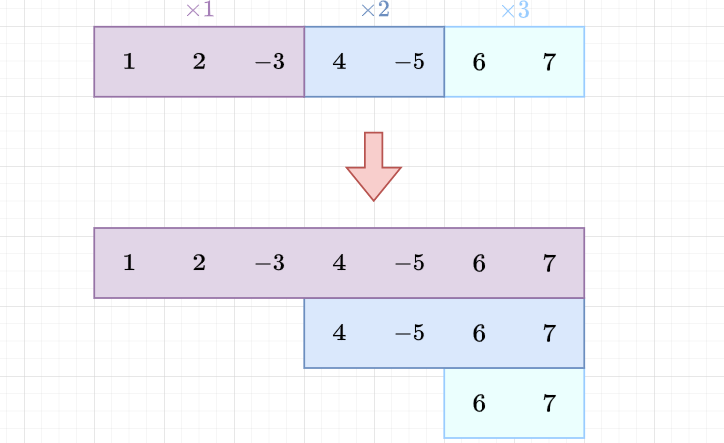
\includegraphics[scale=0.5]{images/array_splitting.png}
    \end{center}
\end{frame}

\begin{frame}
\frametitle{Greedy 題目練習}
    \begin{block}{Codeforces 1175D - Array Splitting}
        你有一個 $n$ 項的陣列 $a_1, a_2, \cdots,a_n$ ,你希望可以將這個陣列,切分為 $k$ 個連續的子陣列子陣列的編號由左到右為 $1$ 到 $k$。定義每個元素的貢獻度為他們的數字乘上他們所在的子陣列編號。換句話說,對於一個在子陣列編號為 $f(i)$ 的數字 $a_i$,他的貢獻度會是 $f(i) \cdot a_i$。請問將這個陣列切分後,貢獻度的總和最多可以是多少? \\
        \vspace{5mm}
        假設陣列是 $[1,2,-3,4,-5,6,-7]$,切成 $[1,2,-3],[4,-5],[6,-7]$,則總貢獻度為 $1 \times 1 + 2 \times 1 + (-3) \times 1 + 4 \times 2 + 5 \times 2 + 6 \times 3 + (-7) \times 3 = -5$ \\
        \vspace{5mm}
        測資範圍: $1 \le n,k \le 3 \times 10^5$
    \end{block}
    \begin{itemize}
        \item<1-> 因此,其實我們會發現,我們只要貪心的拿取最大的後綴和就好了!
        \item<2-> 答案就是整個陣列的總和加上最大的 $k-1$ 個後綴和!
    \end{itemize}
\end{frame}

\begin{frame}
\frametitle{Greedy 題目練習}
    \begin{block}{Codeforces 1203F1 - Complete the Projects (easy version)}
        Koying 在資訊圈十分有名,很多人都會找他合作舉辦活動,而他的名聲目前是 $r$。你知道接下來他會有 $n$ 個邀約,對於每個邀約,只有在 Koying 的名聲在 $a_i$ 以上時,他才能夠接受這個邀約,而經過這次邀約後,他的名聲會改變 $b_i$ (可以是正的也可以是負的)。而在整個過程中,他的名聲不能夠低於 $0$。請問他是否能夠完成這 $n$ 個邀約?
    \end{block}
    \begin{itemize}
        \item<2-> 同樣,我們先留一點時間給大家想想看,有想法的都可以提出來
    \end{itemize}
\end{frame}

\begin{frame}
\frametitle{Greedy 題目練習}
    \begin{block}{Codeforces 1203F1 - Complete the Projects (easy version)}
        Koying 在資訊圈十分有名,很多人都會找他合作舉辦活動,而他的名聲目前是 $r$。你知道接下來他會有 $n$ 個邀約,對於每個邀約,只有在 Koying 的名聲在 $a_i$ 以上時,他才能夠接受這個邀約,而經過這次邀約後,他的名聲會改變 $b_i$ (可以是正的也可以是負的)。而在整個過程中,他的名聲不能夠低於 $0$。請問他是否能夠完成這 $n$ 個邀約?
    \end{block}
    \begin{itemize}
        \item<1-> 首先,這題的難點應該是在 $b_i$ 有可能是負的吧,那我們先將 $b_i$ 為正負的兩種情況分開考慮
        \item<2-> 在 $b_i$ 是正的時候,我們直接從 $a_i$ 小的開始做,一路去完成就好了!
        \item<3-> 那 $b_i$ 是負的時候呢? 
        \item<4-> 我們從大的 $a_i$ 開始處理就好了!
        \item<5-> 先別急! 我們是不是少考慮了什麼條件?
        \item<6-> 名聲不能夠低於 $0$!
    \end{itemize}
\end{frame}

\begin{frame}
\frametitle{Greedy 題目練習}
    \begin{block}{Codeforces 1203F1 - Complete the Projects (easy version)}
        Koying 在資訊圈十分有名,很多人都會找他合作舉辦活動,而他的名聲目前是 $r$。你知道接下來他會有 $n$ 個邀約,對於每個邀約,只有在 Koying 的名聲在 $a_i$ 以上時,他才能夠接受這個邀約,而經過這次邀約後,他的名聲會改變 $b_i$ (可以是正的也可以是負的)。而在整個過程中,他的名聲不能夠低於 $0$。請問他是否能夠完成這 $n$ 個邀約?
    \end{block}
    \begin{itemize}
        \item<1-> 在處理 $b_i$ 是負的時候,我們不能照 $a_i$ 由大到小排序,而應該以 $\max(a_i,-b_i)$ 來進行排序
        \item<2-> 會是 $\max(a_i,-b_i)$ 的原因是因為名聲至少要是 $-b_i$ 以上才能夠接受邀約
        \item<3-> 因此這題的做法就是
            \begin{enumerate}
                \item 先處理 $b_i$ 是正的情況,再處理 $b_i$ 是負的情況
                \item 在 $b_i$ 是正的時候,我們直接將 $a_i$ 由小到大依序完成
                \item 在 $b_i$ 是負的時候,我們照 $\max(a_i,-b_i)$ 由大到小排序
                \item 在過程中只要有任何情況無法接受邀約,答案就是做不到,否則可以完成
            \end{enumerate}
    \end{itemize}
\end{frame}

\begin{frame}
\frametitle{Greedy 題目練習}
    \begin{block}{Codeforces 767E - Change-Free}
        在某個幣值只有 $100$ 元紙鈔與 $1$ 元硬幣的國家,有個旅人 Koying 要在該國生活 $n$ 天,而他一開始有無限多個 $100$ 元紙鈔和 $m$ 個 $1$ 元。他每天會去商店買東西,在第 $i$ 天時,他總共會花 $a_i$ 元購買商品。不過商店的收銀員 Colten 十分討厭找錢,在第 $i$ 天,Colten 會有 $w_i$ 的煩躁度,只要他找了錢,他當天怒氣值就會是 (總共找的紙鈔與硬幣數量 $\times w_i$)。請問 Koying 最小可以讓 Colten 這 $n$ 天的怒氣值總和為多少,並且輸出 Koying 每天應該要付多少紙鈔和硬幣。
    \end{block}
\end{frame}

\begin{frame}
\frametitle{Greedy 題目練習}
    \begin{block}{Codeforces 767E - Change-Free}
        在某個幣值只有 $100$ 元紙鈔與 $1$ 元硬幣的國家,有個旅人 Koying 要在該國生活 $n$ 天,而他一開始有無限多個 $100$ 元紙鈔和 $m$ 個 $1$ 元。他每天會去商店買東西,在第 $i$ 天時,他總共會花 $a_i$ 元購買商品。不過商店的收銀員 Colten 十分討厭找錢,在第 $i$ 天,Colten 會有 $w_i$ 的煩躁度,只要他找了錢,他當天怒氣值就會是 (總共找的紙鈔與硬幣數量 $\times w_i$)。請問 Koying 最小可以讓 Colten 這 $n$ 天的怒氣值總和為多少,並且輸出 Koying 每天應該要付多少紙鈔和硬幣。
    \end{block}
    \begin{itemize}
        \item<1-> 這題的想法有點難度,也讓大家稍微想想看,有想法都可以提出來
    \end{itemize}
\end{frame}

\begin{frame}
\frametitle{Greedy 題目練習}
    \begin{itemize}
        \item<1-> 首先,我們要想想看,我們有可能怎麼樣付錢呢?
        \item<2-> 在第 $i$ 天,我們有以下兩種付錢的可能性:
            \begin{enumerate}
                \item 付 $\lfloor \frac{c_i}{100} \rfloor$ 個紙鈔和 $c_i \bmod 100$ 個硬幣
                \item 付 $\lceil \frac{c_i}{100} \rceil$ 個紙鈔
            \end{enumerate}
        \item<3-> 選擇以上兩個方案時,找的錢分別為: 
            \begin{enumerate}
                \item 找 $0$ 元
                \item 找 $100 - c_i \bmod 100$ 元
            \end{enumerate}
        \item<4-> 那麼我們可以發現,對於某一天,假設我們選擇了第二種,則 Colten 的怒氣值會增加 $w_i \times (100 - c_i \bmod 100)$
    \end{itemize}
\end{frame}

\begin{frame}
\frametitle{Greedy 題目練習}
    \begin{itemize}
        \item<1-> 因此,對於本題,我們可以依序考慮每一天
        \item<2-> 對於第 $i$ 天,如果當前的硬幣數量 $> c_i \bmod 100$,那我們可以選擇直接用第一種付錢方案
        \item<2-> 否則,我們可以考慮將前 $i$ 天選擇了第一種付錢方案的人且改成第二種時增加的怒氣值最少的改成方案二
        \item<3-> 以上的想法,我們可以使用 priority\_queue 完成!
    \end{itemize}
\end{frame}

\begin{frame}
\frametitle{Greedy 題目練習}
    \begin{block}{Codeforces 449C - Jzzhu and Apples}
        你有 $1$ 到 $n$ 的數字,你可以選兩個不互質的數字組成一組,請問你最多可以選出幾組?
    \end{block}
    \begin{itemize}
        \item<2-> 想想看有什麼性質是可以利用的!
        \item<3-> 偶數很多!
    \end{itemize}
\end{frame}

\begin{frame}
\frametitle{Greedy 題目練習}
    \begin{block}{Codeforces 449C - Jzzhu and Apples}
        你有 $1$ 到 $n$ 的數字,你可以選兩個不互質的數字組成一組,請問你最多可以選出幾組?
    \end{block}
    \begin{itemize}
        \item<1-> 首先,我們先從質數 $p$ 的倍數開始下手
        \item<2-> 對於一個質數 $p \ge 3$,我們依序枚舉 $p,2p,3p,\ldots$,然後試著將兩兩配在一起
        \item<3-> 如果總共有奇數個,則我們考慮將數字中的偶數留下
        \item<4-> 當我們配完所有質數的倍數之後,我們再將沒用過的偶數倆倆配在一起!
        \item<5-> 這樣貪心的去配,這題就做完了!
    \end{itemize}
\end{frame}

\section{總結}

\begin{frame}
\frametitle{總結}
    \begin{itemize}
        \item 經過這堂課,希望大家對於 Greedy 有了更深的了解
        \item 這個技巧,在比賽當中,一般會是用猜的來得到做法
        \item 而這堂課我們不只是介紹了這些猜測的作法,也教給各位一些證明的方式
        \item 未來大家也會遇到很多種不同的 Greedy 題目,將這堂課所教的內容學起來的話,應該能夠有不少收穫
    \end{itemize}
\end{frame}

% Codeforces 449C

\end{document}